\documentclass[11pt,a4paper,]{article}
\usepackage{lmodern}

\usepackage{amssymb,amsmath}
\usepackage{ifxetex,ifluatex}
\usepackage{fixltx2e} % provides \textsubscript
\ifnum 0\ifxetex 1\fi\ifluatex 1\fi=0 % if pdftex
  \usepackage[T1]{fontenc}
  \usepackage[utf8]{inputenc}
\else % if luatex or xelatex
  \usepackage{unicode-math}
  \defaultfontfeatures{Ligatures=TeX,Scale=MatchLowercase}
\fi
% use upquote if available, for straight quotes in verbatim environments
\IfFileExists{upquote.sty}{\usepackage{upquote}}{}
% use microtype if available
\IfFileExists{microtype.sty}{%
\usepackage[]{microtype}
\UseMicrotypeSet[protrusion]{basicmath} % disable protrusion for tt fonts
}{}
\PassOptionsToPackage{hyphens}{url} % url is loaded by hyperref
\usepackage[unicode=true]{hyperref}
\hypersetup{
            pdftitle={Loney Meadow Restoration Project Monitoring: Loney Meadow Amphibian Surveys 2019},
            pdfborder={0 0 0},
            breaklinks=true}
\urlstyle{same}  % don't use monospace font for urls
\usepackage{geometry}
\geometry{a4paper, centering, text={16cm,24cm}}
\usepackage[style=authoryear-comp,]{biblatex}
\addbibresource{paperpile\_amphibs.bib}
\usepackage{longtable,booktabs}
% Fix footnotes in tables (requires footnote package)
\IfFileExists{footnote.sty}{\usepackage{footnote}\makesavenoteenv{long table}}{}
\IfFileExists{parskip.sty}{%
\usepackage{parskip}
}{% else
\setlength{\parindent}{0pt}
\setlength{\parskip}{6pt plus 2pt minus 1pt}
}
\setlength{\emergencystretch}{3em}  % prevent overfull lines
\providecommand{\tightlist}{%
  \setlength{\itemsep}{0pt}\setlength{\parskip}{0pt}}
\setcounter{secnumdepth}{0}

% set default figure placement to htbp
\makeatletter
\def\fps@figure{htbp}
\makeatother


\title{Loney Meadow Restoration Project Monitoring: Loney Meadow Amphibian Surveys 2019}

%% CWS STUFF

%% CAPTIONS
\RequirePackage{caption}
\DeclareCaptionStyle{italic}[justification=centering]
 {labelfont={bf},textfont={it},labelsep=colon}
\captionsetup[figure]{style=italic,format=hang,singlelinecheck=true}
\captionsetup[table]{style=italic,format=hang,singlelinecheck=true}


%% FONT
\RequirePackage{bera}
\RequirePackage[charter,expert,sfscaled]{mathdesign}
\RequirePackage{fontawesome}

%% HEADERS AND FOOTERS
\RequirePackage{fancyhdr}
\pagestyle{fancy}
\rfoot{\Large\sffamily\raisebox{-0.1cm}{\textbf{\thepage}}}
\makeatletter
\lhead{\textsf{\expandafter{\@title}}}
\makeatother
\rhead{}
\cfoot{}
\setlength{\headheight}{15pt}
\renewcommand{\headrulewidth}{0.4pt}
\renewcommand{\footrulewidth}{0.4pt}
\fancypagestyle{plain}{%
\fancyhf{} % clear all header and footer fields
\fancyfoot[C]{\sffamily\thepage} % except the center
\renewcommand{\headrulewidth}{0pt}
\renewcommand{\footrulewidth}{0pt}}

%% MATHS
\RequirePackage{bm,amsmath}
\allowdisplaybreaks

%% GRAPHICS
\RequirePackage{graphicx}
\setcounter{topnumber}{2}
\setcounter{bottomnumber}{2}
\setcounter{totalnumber}{4}
\renewcommand{\topfraction}{0.85}
\renewcommand{\bottomfraction}{0.85}
\renewcommand{\textfraction}{0.15}
\renewcommand{\floatpagefraction}{0.8}


%\RequirePackage[section]{placeins}

%% SECTION TITLES


%% SECTION TITLES
\RequirePackage[compact,sf,bf]{titlesec}
\titleformat*{\section}{\Large\sf\bfseries\color[rgb]{0.03, 0.27, 0.49}}
\titleformat*{\subsection}{\large\sf\bfseries\color[rgb]{0.03, 0.27, 0.49}}
\titleformat*{\subsubsection}{\sf\bfseries\color[rgb]{0.03, 0.27, 0.49}}
\titlespacing{\section}{0pt}{2ex}{.5ex}
\titlespacing{\subsection}{0pt}{1.5ex}{0ex}
\titlespacing{\subsubsection}{0pt}{.5ex}{0ex}


%% TITLE PAGE
\def\Date{\number\day}
\def\Month{\ifcase\month\or
 January\or February\or March\or April\or May\or June\or
 July\or August\or September\or October\or November\or December\fi}
\def\Year{\number\year}

%% LINE AND PAGE BREAKING
\sloppy
\clubpenalty = 10000
\widowpenalty = 10000
\brokenpenalty = 10000
\RequirePackage{microtype}

%% PARAGRAPH BREAKS
\setlength{\parskip}{1.4ex}
\setlength{\parindent}{0em}

%% HYPERLINKS
\RequirePackage{xcolor} % Needed for links
\definecolor{airforceblue}{rgb}{0.36, 0.54, 0.66}
\definecolor{cerulean}{rgb}{0.0, 0.48, 0.65}
\definecolor{darkcerulean}{rgb}{0.03, 0.27, 0.49}
\RequirePackage{url}

\makeatletter
\@ifpackageloaded{hyperref}{}{\RequirePackage{hyperref}}
\makeatother
\hypersetup{
     citecolor=0 0 0,
     hidelinks=true,
     breaklinks=true,
     bookmarksopen=true,
     bookmarksnumbered=true,
     linkcolor=darkcerulean,
     urlcolor=darkcerulean,
     citecolor=darkcerulean,
     colorlinks=true}

\usepackage[showonlyrefs]{mathtools}
\usepackage[no-weekday]{eukdate}

%% BIBLIOGRAPHY

\makeatletter
\@ifpackageloaded{biblatex}{}{\usepackage[style=authoryear-comp, backend=biber, natbib=true]{biblatex}}
\makeatother
\ExecuteBibliographyOptions{bibencoding=utf8,minnames=1,maxnames=3, maxbibnames=99,dashed=false,terseinits=true,giveninits=true,uniquename=false,uniquelist=false,doi=false, isbn=false,url=true,sortcites=false}

\DeclareFieldFormat{url}{\texttt{\url{#1}}}
\DeclareFieldFormat[article]{pages}{#1}
\DeclareFieldFormat[inproceedings]{pages}{\lowercase{pp.}#1}
\DeclareFieldFormat[incollection]{pages}{\lowercase{pp.}#1}
\DeclareFieldFormat[article]{volume}{\mkbibbold{#1}}
\DeclareFieldFormat[article]{number}{\mkbibparens{#1}}
\DeclareFieldFormat[article]{title}{\MakeCapital{#1}}
\DeclareFieldFormat[article]{url}{}
%\DeclareFieldFormat[book]{url}{}
%\DeclareFieldFormat[inbook]{url}{}
%\DeclareFieldFormat[incollection]{url}{}
%\DeclareFieldFormat[inproceedings]{url}{}
\DeclareFieldFormat[inproceedings]{title}{#1}
\DeclareFieldFormat{shorthandwidth}{#1}
%\DeclareFieldFormat{extrayear}{}
% No dot before number of articles
\usepackage{xpatch}
\xpatchbibmacro{volume+number+eid}{\setunit*{\adddot}}{}{}{}
% Remove In: for an article.
\renewbibmacro{in:}{%
  \ifentrytype{article}{}{%
  \printtext{\bibstring{in}\intitlepunct}}}

\AtEveryBibitem{\clearfield{month}}
\AtEveryCitekey{\clearfield{month}}

\makeatletter
\DeclareDelimFormat[cbx@textcite]{nameyeardelim}{\addspace}
\makeatother

\author{\sf\Large\textbf{ Dr Ryan Peek}\\ {\sf\large Postdoctoral Scholar\\[0.5cm]}}

\date{\sf\Date~\Month~\Year}
\makeatletter
\lfoot{\sf Ryan Peek: \@date}
\makeatother


%%%% PAGE STYLE FOR FRONT PAGE OF REPORTS

\makeatletter
\def\organization#1{\gdef\@organization{#1}}
\def\telephone#1{\gdef\@telephone{#1}}
\def\email#1{\gdef\@email{#1}}
\makeatother
  \organization{SYRCL}

  \def\name{Center for\newline Watershed Sciences}

  \telephone{530.754.9133}

  \email{rapeek@ucdavis.edu}

\def\webaddress{\url{https://watershed.ucdavis.edu/}}
\def\logo{
\includegraphics[width=6cm]{CWSAltDesign}}
\def\extraspace{\vspace*{1.6cm}}
\makeatletter
\def\contactdetails{\faicon{phone} & \@telephone \\
                    \faicon{envelope} & \@email}
\makeatother

%%%% FRONT PAGE OF REPORTS

\def\reporttype{Report for}

\long\def\front#1#2#3{
\newpage
\begin{singlespacing}
\thispagestyle{empty}
\vspace*{-1.4cm}
\hspace*{-1.4cm}
\hbox to 16cm{
  \hbox to 6.5cm{\vbox to 14cm{\vbox to 25cm{
    \logo
    \vfill
    \parbox{6.3cm}{\raggedright
      \sf\color[rgb]{0.00,0.00,0.70}
      {\large\textbf{\name}}\par
      \vspace{.7cm}
      \tabcolsep=0.12cm\sf\small
      \begin{tabular}{@{}ll@{}}\contactdetails
      \end{tabular}
    }
  }\vss}\hss}
  \hspace*{0.2cm}
  \hbox to 1cm{\vbox to 14cm{\rule{1pt}{26.8cm}\vss}\hss\hfill}
  \hbox to 10cm{\vbox to 14cm{\vbox to 25cm{
      \vspace*{3cm}\sf\raggedright
      \parbox{11cm}{\sf\raggedright\baselineskip=1.2cm
         \fontsize{24.88}{30}\color[rgb]{0, 0, 0}\sf\textbf{#1}}
      \par
      \vfill
      \large
      \vbox{\parskip=0.8cm #2}\par
      \vspace*{2cm}\par
      \reporttype\\[0.3cm]
      \hbox{#3}%\\[2cm]\
      \vspace*{1cm}
      {\large\sf\textbf{\Date~\Month~\Year}}
   }\vss}
  }}
\end{singlespacing}
\newpage
}

\makeatletter
\def\titlepage{\front{\expandafter{\@title}}{\@author}{\@organization}}
\makeatother

\usepackage{setspace}
\setstretch{1.2}

%% Any special functions or other packages can be loaded here.
\usepackage{booktabs}
\usepackage{longtable}
\usepackage{array}
\usepackage{multirow}
\usepackage{wrapfig}
\usepackage{float}
\usepackage{colortbl}
\usepackage{pdflscape}
\usepackage{tabu}
\usepackage{threeparttable}
\usepackage{threeparttablex}
\usepackage[normalem]{ulem}
\usepackage{makecell}
\usepackage{xcolor}


\begin{document}
\titlepage

\hypertarget{overview}{%
\subsection{OVERVIEW}\label{overview}}

Loney Meadow and the surrounding meadow complex were surveyed for the presence of amphibian species of interest as part of amphibian monitoring in the Loney Meadow area prior/post to stream bank restoration activities. Surveys were conducted throughout Loney Meadow and at several adjacent lentic features to determine presence and life stages of sensitive amphibian species. Observations were compared across surveys from pre and post meadow restoration activities. Repeat visual encounter surveys were conducted prior to restoration in June of 2015 and July of 2016, and post restoration surveys were conducted in July and August of 2019.

\begin{figure}

{\centering \includegraphics[width=0.7\linewidth]{/Users/ryanpeek/Documents/github/loney_mdw/figs/P1160425} 

}

\caption{Surveys in Main Meadow}\label{fig:fig1}
\end{figure}

\hypertarget{methods}{%
\subsection{METHODS}\label{methods}}

Meadow and stream channel surveys were conducted in Loney Meadow following survey protocols in \textcite{Heyer1994-dr}. Both day and night surveys were conducted with four surveyors using combined methods such as visual observation, dip netting, and auditory surveys to maximize potential detection of herpetofauna. During each survey, surveyors walked across the meadow at equal intervals, zig-zagging along a transect corresponding to the longest meadow axis. All visible and accessible stream channels were also walked in pairs or in groups of three, with surveyors on each bank and one or two surveyors in the channel. In both the meadow and stream channels, surveyors used dipnets and D-nets to sweep vegetation and aquatic habitat for individuals. Upon observation of species, locations were marked and survey time was stopped during processing and identification. Survey effort was calculated for each survey by the total survey time multiplied by the number of surveyors. Prior to and following surveys, all equipment and field gear was decontaminated following accepted protocols \autocite{Daszak2001-in,Johnson2003-yc,Phillott2010-mt}. All analysis and mapping was conducted in R using \texttt{tidyverse}, \texttt{sf} and \texttt{ggmap} packages \autocite{Kahle2013-rh,Pebesma2018-vd,R_Core_Team2019-pk,Wickham2019-zw}.

\hypertarget{sites}{%
\subsection{SITES}\label{sites}}

In 2019, Loney Meadow and several adjacent lentic ponds or lake habitats were surveyed during July and August (Figure \ref{fig:fig1}, Figure \ref{fig:fig2}). Each site was visited during clear and sunny conditions. The stockpond, Bullpen Lake, and unnamed pond (NE) and (E) did not appear to have changed in structure or condition between visits, and since previous visits in 2016.

\begin{figure}

{\centering 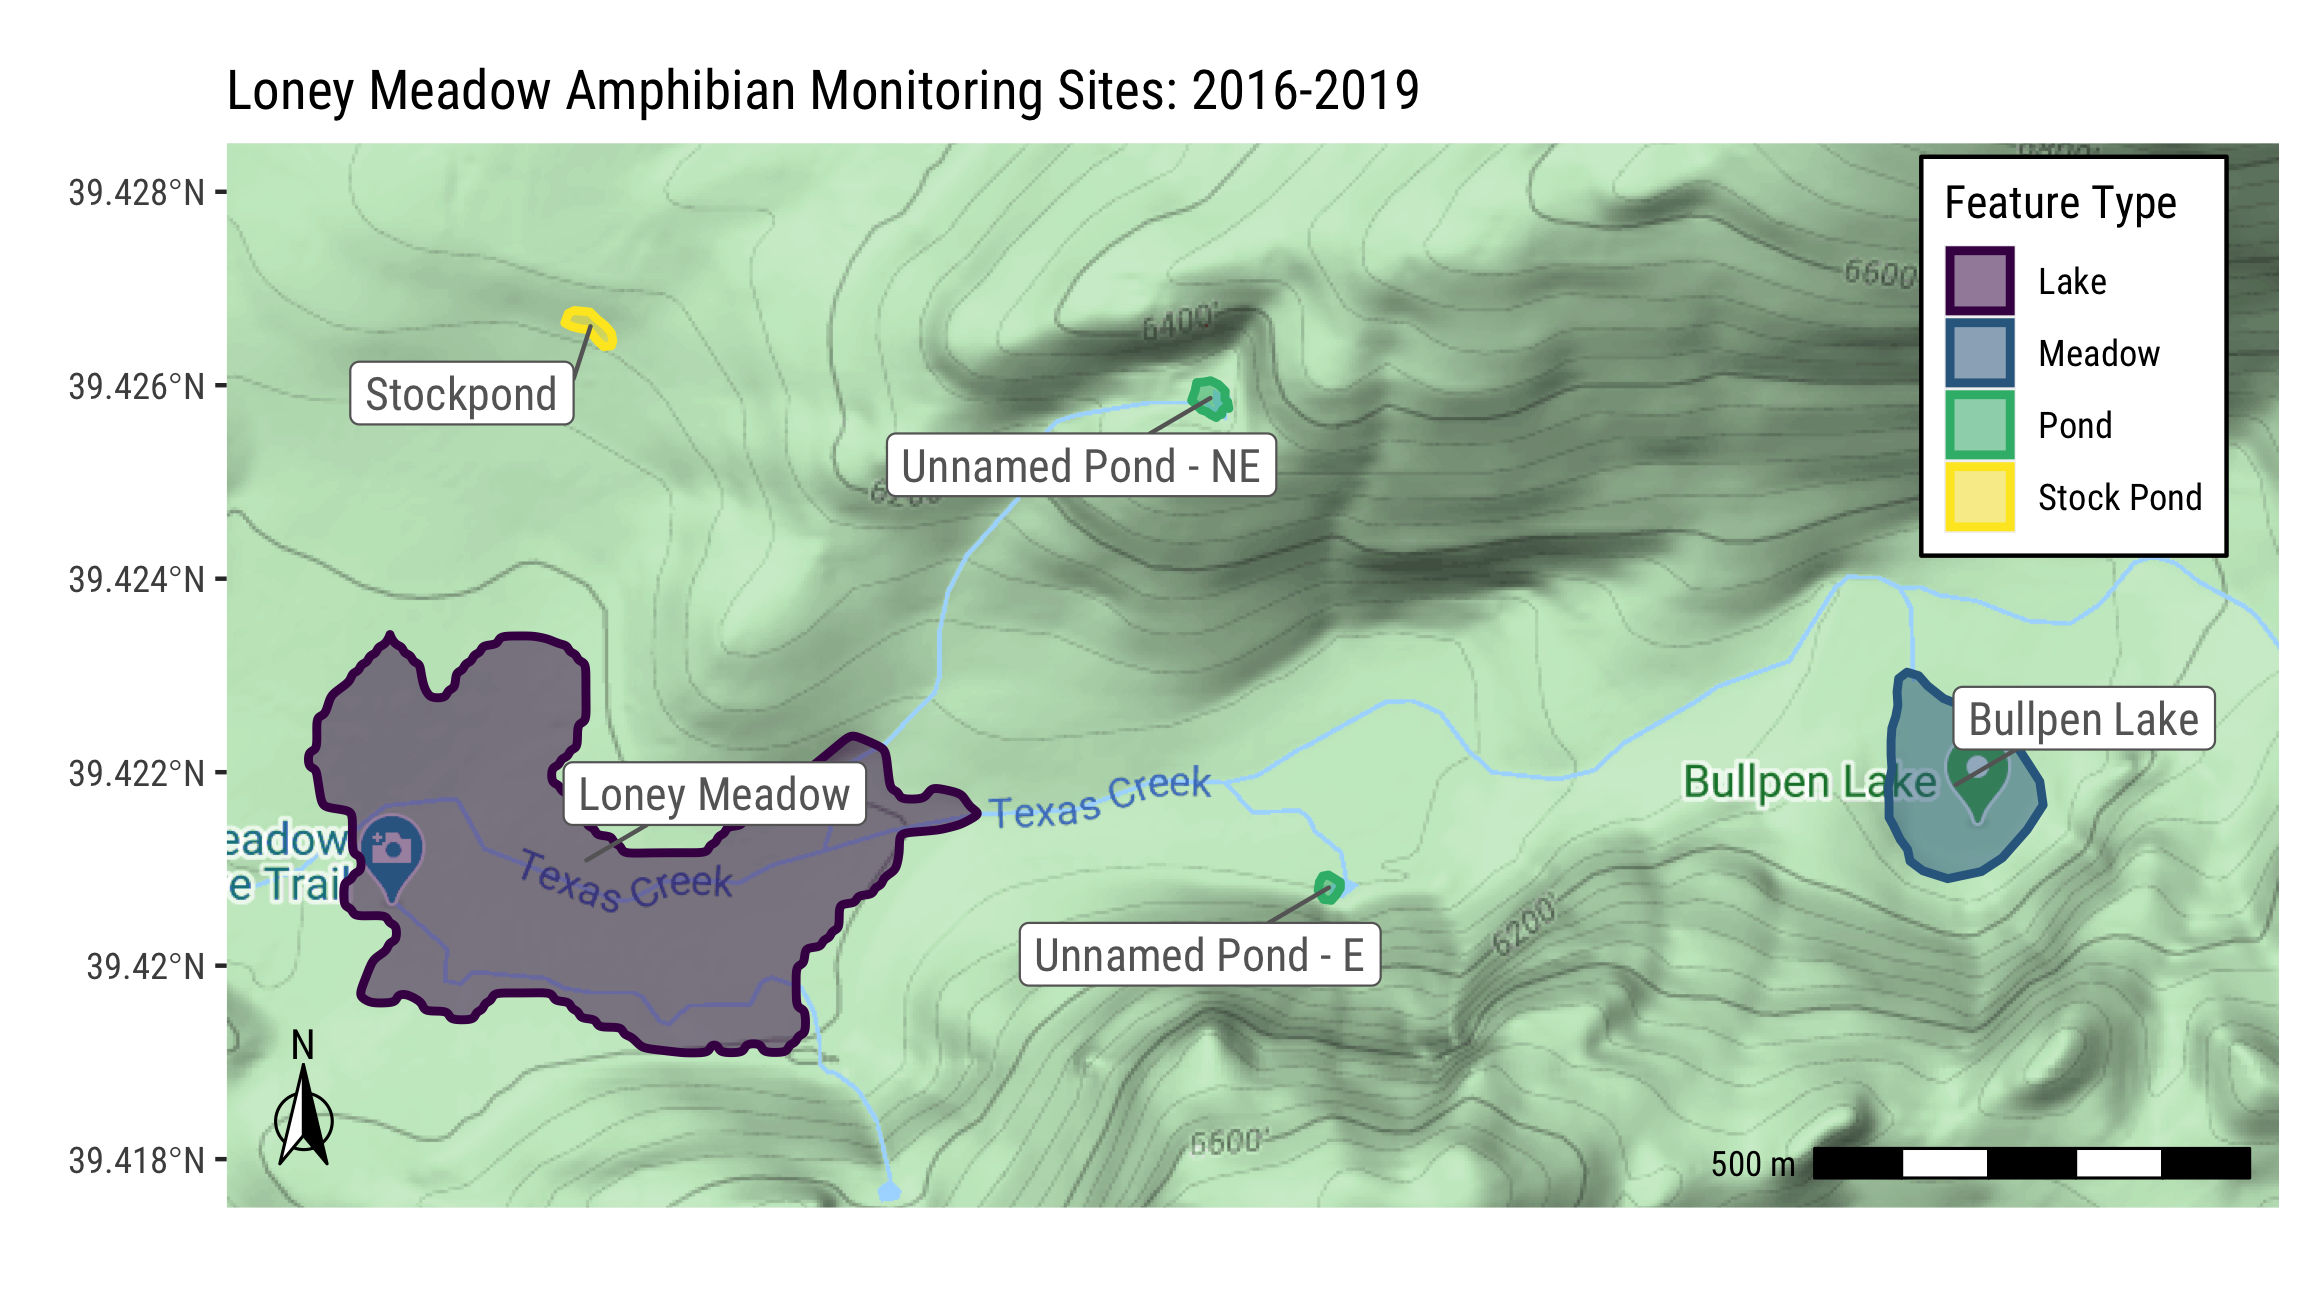
\includegraphics[width=1\linewidth]{/Users/ryanpeek/Documents/github/loney_mdw/figs/final_map_sites} 

}

\caption{Map of Survey Sites}\label{fig:fig2}
\end{figure}

The ponds surveyed surrounding Loney Meadow appear to remain largely permanent, though the water levels fluctuate depending on the month surveyed (see Figure \ref{fig:fig3} and Figure \ref{fig:fig4}). These habitats may provide refugia and suitable sources for amphibian populations, and occur within distances feasible for amphibian movement. Centroid distance from \textbf{Loney Meadow} to \textbf{Bullpen Lake} is approximately 0.98 miles, while centroid distance between Loney Meadow and the \textbf{Unnamed Pond - East} is 0.55 miles.

\begin{figure}

{\centering \includegraphics[width=0.7\linewidth]{/Users/ryanpeek/Documents/github/loney_mdw/figs/P1160447} 

}

\caption{Lentic unnamed pond east of Loney Meadow in August 2019, looking southeast}\label{fig:fig3}
\end{figure}

\begin{figure}

{\centering \includegraphics[width=0.7\linewidth]{/Users/ryanpeek/Documents/github/loney_mdw/figs/P1080273} 

}

\caption{Lentic unnamed pond east of Loney Meadow in July 2016, looking southeast}\label{fig:fig4}
\end{figure}

\hypertarget{results}{%
\subsection{RESULTS}\label{results}}

Surveys for amphibians were conducted in Loney Meadow on July 16 and August 21, 2019 (Table 1). Teams of two or three observers walked along wetted perimeters, stream corridors, and four or more observers were used in wet meadow areas with no clear channel.

\begin{table}

\caption{\label{tab:table1}2019 Surveys}
\centering
\begin{tabular}[t]{l|r|r|r|r|l|r}
\hline
Site & Start Time & End Time & Surveyors & Effort (min) & Conditions & Month\\
\hline
Loney Meadow & 1101 & 1430 & 7 & 1883 & Clear, Sunny & 7\\
\hline
Unnamed Pond & 1522 & 1430 & 7 & 686 & Clear, Sunny & 7\\
\hline
Loney Meadow & 900 & 1107 & 4 & 468 & Clear, Sunny & 8\\
\hline
Unnamed Pond & 1153 & 1300 & 4 & 588 & Clear, sunny & 8\\
\hline
\end{tabular}
\end{table}

\hypertarget{amphibians}{%
\subsubsection{Amphibians}\label{amphibians}}

In 2019, surveys found primarily Pacific chorus frogs (\emph{Pseudacris regilla}) {[}PSRE{]} in multiple life stages (eggs, tadpoles and adults were observed), however, Southern long-toed salamanders (\emph{Ambystoma macrodactylum sigillatum}) {[}AMMASI{]} larvae were observed again in the small pond just northeast of the main Loney Meadow (Figure \ref{fig:fig3} and Figure \ref{fig:fig5}). This is the same location they were observed in 2016 as well. The AMMASI larvae were observed at an elevation approximately 100 meters higher than Loney Meadow, and have consistently been observed at this site since 2016. No other site at or near Loney Meadow has detected AMMASI. There was no evidence of grazing or cattle at the unnamed pond. Additional herpetofauna observed in 2019 included Sierra and mountain gartersnakes (\emph{Thamnophis couchii} {[}THCO{]} and \emph{Thamnophis elegans elegans} {[}THEL{]}). Both of these species were observed in multiple locations within the area, similar to 2015 and 2016. There were no new species observed in 2019 that were not observed in 2015 or 2016.

\begin{figure}

{\centering 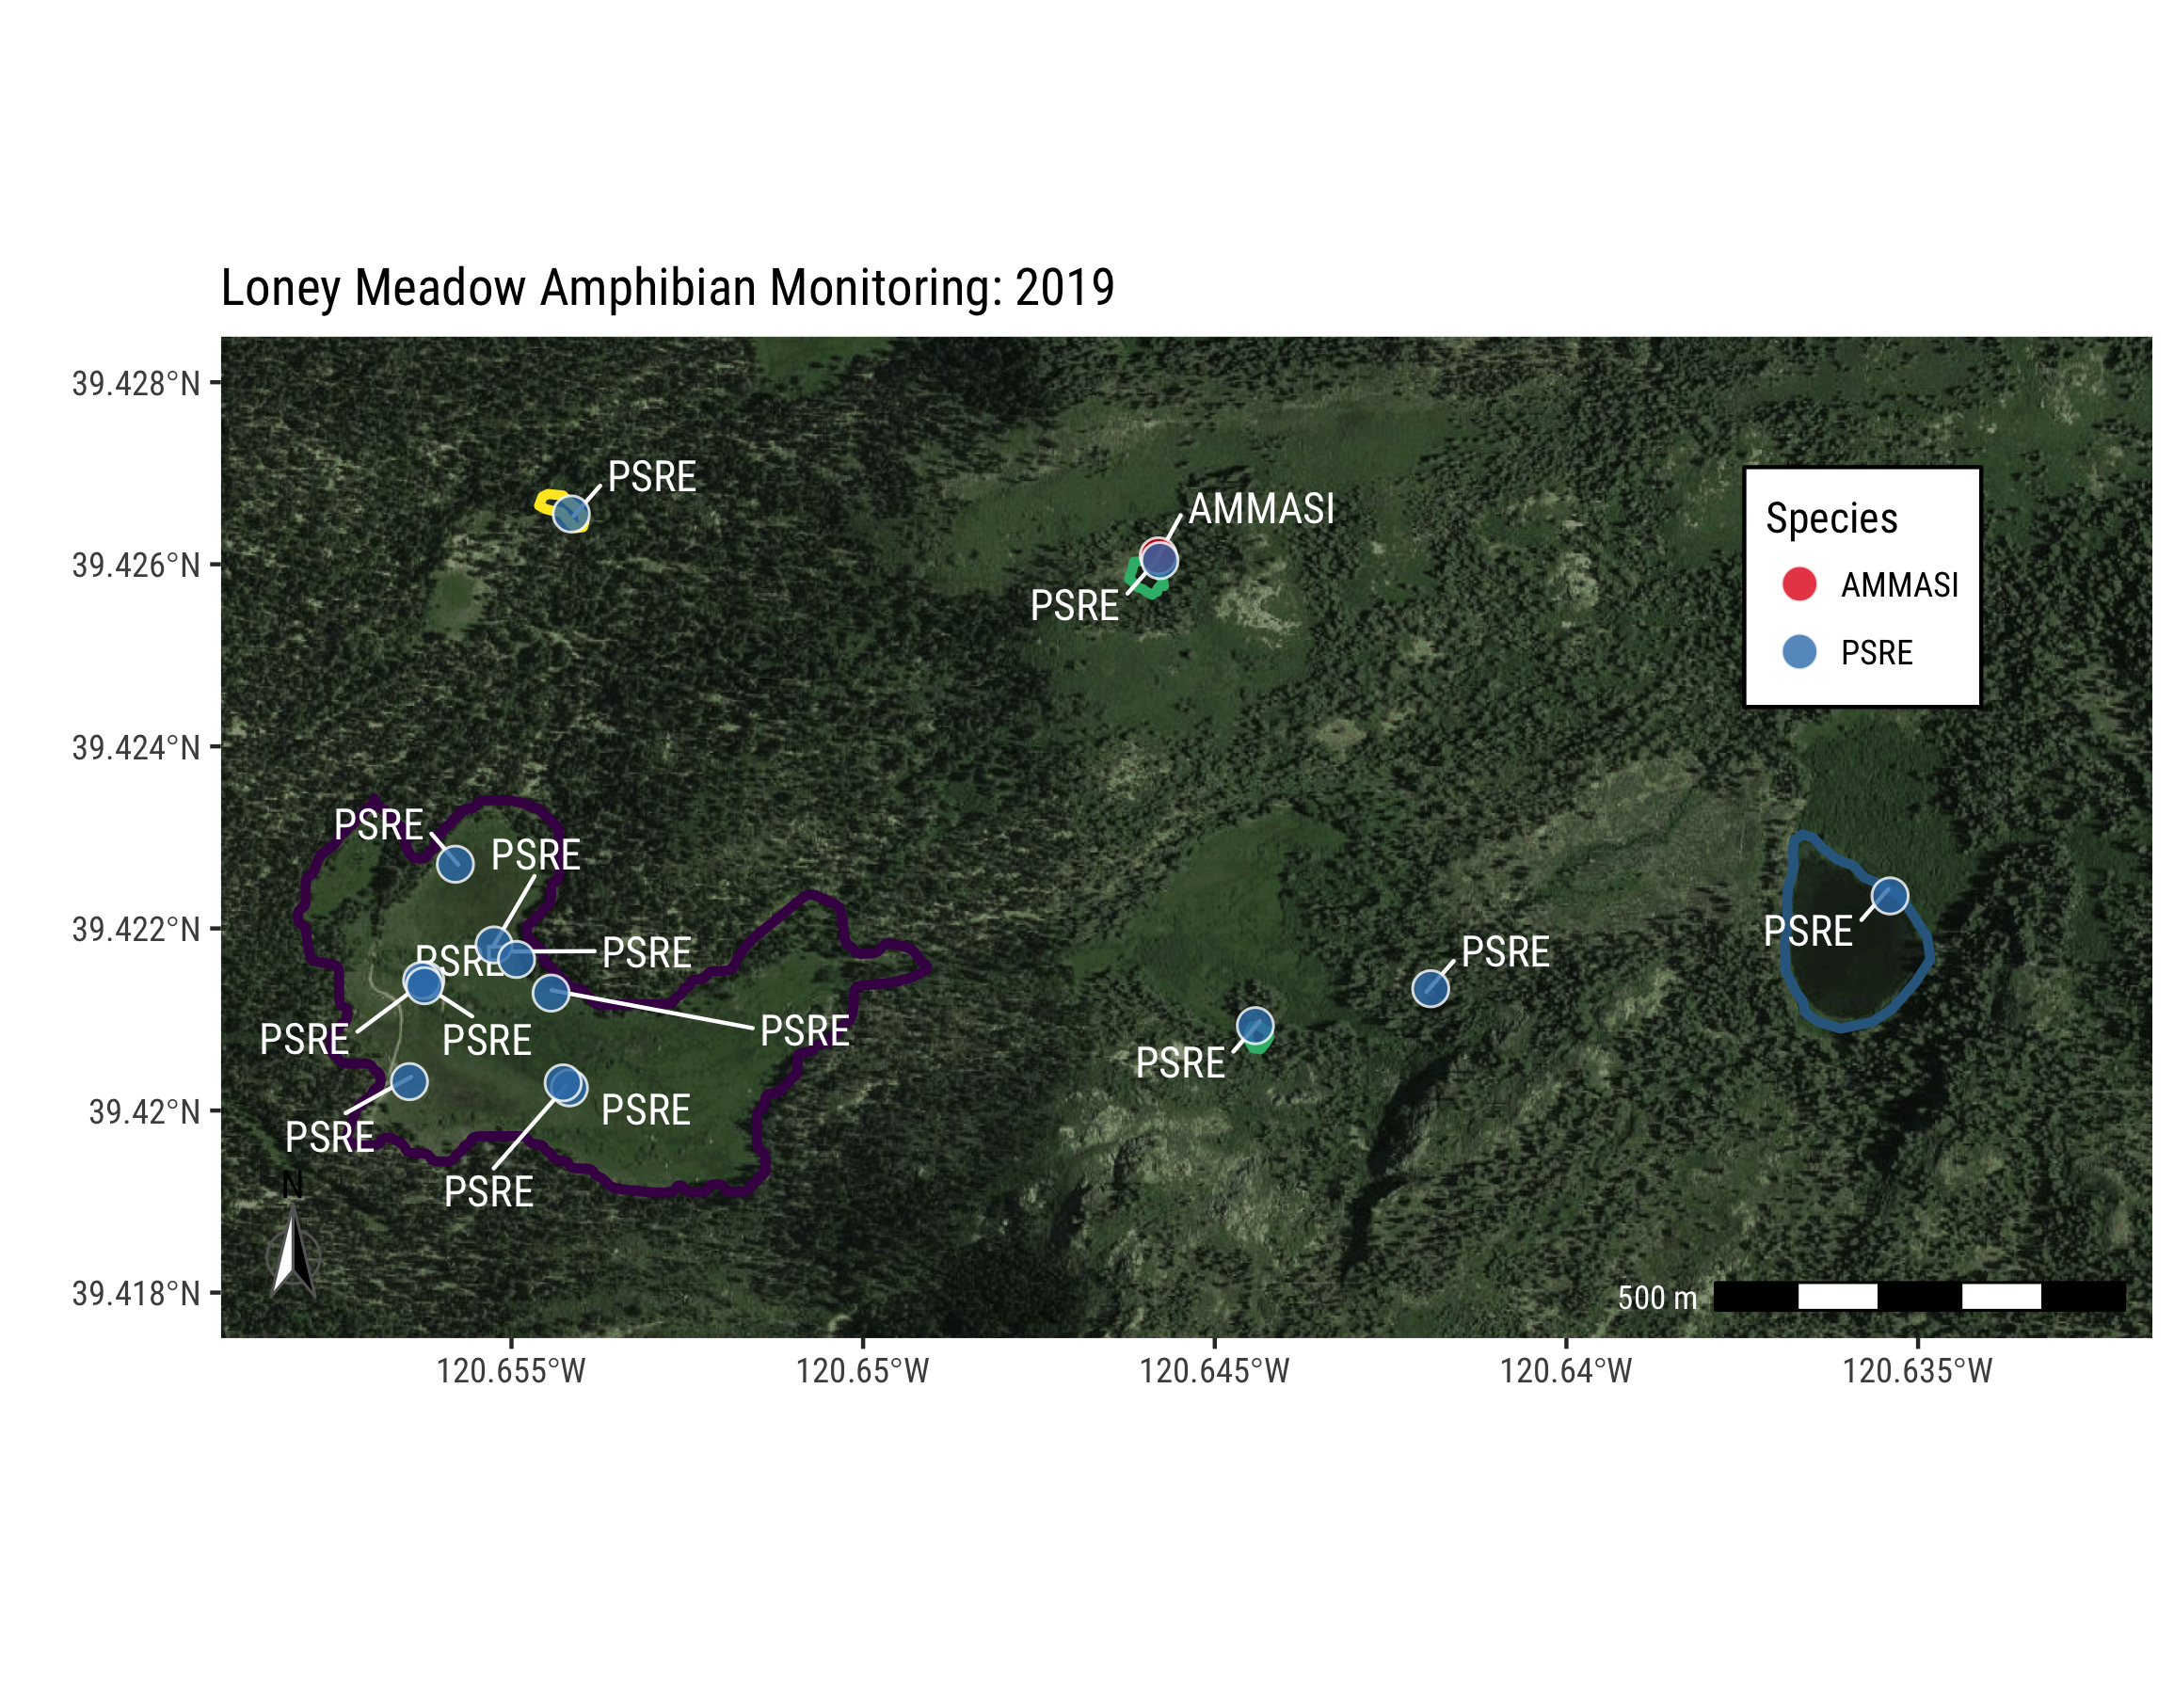
\includegraphics[width=1\linewidth]{/Users/ryanpeek/Documents/github/loney_mdw/figs/final_map_2019_obs} 

}

\caption{Map of amphibian species observations 2019.}\label{fig:fig5}
\end{figure}

\begin{longtable}[t]{l|l|l|l|r|r|l}
\caption{\label{tab:table2}2019 Observations}\\
\hline
\textbf{Species} & \textbf{Species Code} & \textbf{Stage} & \textbf{No. Obs} & \textbf{UTM E} & \textbf{UTM N} & \textbf{Month}\\
\hline
\hline
Thamnophis couchii & THCO & Adult & 1 & 701749 & 4366162 & July\\
\hline
Pseudacris regilla & PSRE & Larvae & 10 & 701749 & 4366162 & July\\
\hline
Ambystoma macrodactylum sigillatum & AMMASI & Larvae & 60 & 702633 & 4366699 & July\\
\hline
Pseudacris regilla & PSRE & Larvae & >100 & 702633 & 4366699 & July\\
\hline
Pseudacris regilla & PSRE & Larvae & 3 & 701860 & 4366204 & August\\
\hline
Pseudacris regilla & PSRE & Larvae & 10 & 701929 & 4366042 & August\\
\hline
Pseudacris regilla & PSRE & Adult & 3 & 701929 & 4366042 & August\\
\hline
Pseudacris regilla & PSRE & Larvae & >100 & 702633 & 4366699 & August\\
\hline
Ambystoma macrodactylum sigillatum & AMMASI & Larvae & >100 & 702633 & 4366699 & August\\
\hline
Fairy Shrimp & NA & Larvae & 5 & 702633 & 4366699 & August\\
\hline
Thamnophis couchii & THCO & Adult & 4 & 702633 & 4366699 & August\\
\hline
\end{longtable}

\pagebreak

\begin{figure}

{\centering \includegraphics[width=0.7\linewidth]{/Users/ryanpeek/Documents/github/loney_mdw/figs/P1160459} 

}

\caption{Pacific chorus frog in unnamed pond (northeast)}\label{fig:fig6}
\end{figure}

\begin{figure}

{\centering \includegraphics[width=0.7\linewidth]{/Users/ryanpeek/Documents/github/loney_mdw/figs/P1090885} 

}

\caption{Sierra garter snake in Loney Meadow}\label{fig:fig7}
\end{figure}

\begin{figure}

{\centering \includegraphics[width=0.7\linewidth]{/Users/ryanpeek/Documents/github/loney_mdw/figs/P1160474} 

}

\caption{Southern long-toed salamander larvae in unnamed pond (northeast)}\label{fig:fig8}
\end{figure}

\hypertarget{additional-observations}{%
\subsubsection{Additional Observations}\label{additional-observations}}

In addition to herpetofauna observed in 2019, we observed spinytail fairy shrimp (\emph{Streptocephalus sealli}) (see \textcite{Dexter1956-yl}) in the unnamed pond (NE). Several of these shrimp were observed in the pond along the margins in the same areas the Southern long-toed salamanders were observed (Figure \ref{fig:fig9}). These species are not listed and and are the most widely distributed fairy shrimp in North America \autocite{Eriksen1999-qk}. Fairy shrimps are well adapted to occurring in habitats that may dessicate via a reproductive strategy which uses cysts. Cysts are highly resistant and stable ``eggs'' by which fairy shrimps reproduce or hatch into nauplii. Interestingly, fairy shrimps are a common prey item of salamanders \autocite{Eriksen1999-qk}. In addition the cysts can be successfully passed through salamander and crayfish digestive systems and remain viable, thus predation does not end the life-cycle of the fairy shrimp \autocite{Eriksen1999-qk}.

\begin{figure}

{\centering \includegraphics[width=0.7\linewidth]{/Users/ryanpeek/Documents/github/loney_mdw/figs/P1160476} 

}

\caption{Spinytail fairy shrimp at unnamed pond (NE)}\label{fig:fig9}
\end{figure}

\begin{figure}

{\centering \includegraphics[width=0.7\linewidth]{/Users/ryanpeek/Documents/github/loney_mdw/figs/P1160481} 

}

\caption{Spinytail fairy shrimp in unnamed pond (NE)}\label{fig:fig10}
\end{figure}

\printbibliography

\end{document}
